\documentclass[ignorenonframetext,compress]{beamer}

\mode<presentation>

\usepackage{times}
\usefonttheme{structurebold}

\usepackage[english]{babel}
\usepackage{tabularx}
\usepackage{url}
\usepackage{zed-csp}
\usepackage{subfigure}
\usepackage{epsfig}
\usepackage{graphicx}
\usepackage{color}

\renewcommand*{\thesubfigure}{}

\usetheme{Madrid}

\title[PODD -- An Ontology-driven Repository]{PODD: An Ontology-driven Data Repository for Collaborative Phenomics Research}

\author[Yuan-Fang Li]{
    \textbf{Yuan-Fang Li}\\
    \url{liyf@itee.uq.edu.au}
    }

\institute[UQ]{
    The eResearch Lab, School of ITEE\\The University of Queensland\\
    }
    
\vspace{+380pt}
\date[ICADL 2010]{\footnotesize $12^{th}$ International Conference on Asian Digital Libraries -- Gold Coast, Australia}

\AtBeginSection[]{\frame{\frametitle{Outline}\tableofcontents[current]}}

\begin{document}

\begin{frame}
    \titlepage
\end{frame}

\part{Main Part}

\section{Introduction}
\begin{frame}{Motivation}
\begin{block}{Challenges in phenomics research data management}
    \begin{itemize}
        \item Data is huge
        \begin{itemize}
%            \item APN: estimated 1.8TB + 30\% growth/year
            \item TPA: 0.5TB/week $\sim 25$ TB/year
        \end{itemize}
        \pause
        \item New platforms/processes/technologies quickly emerge
        \pause
        \item Data needs \textbf{\emph{context}}
        \begin{itemize}
            \item Scientific, administrative \& other metadata
        \end{itemize}
    \end{itemize}
\end{block}
\pause
\begin{block}{Repositories for the management of data}
    \begin{itemize}
      \item Not all questions answered
    \end{itemize}
\end{block}
\end{frame}

There are 3 major challenges to data management in phenomics research.

1. The volume of data. Phenomics research generates large amounts of
data. For example, The Plant Accelerator, one of the research centers
in Australian Plant Phenomics Facility, is
estimated to generate 25TB of data per year. And TPA is only one
research center. Under APPF there is still the High-resolution Plant
Phenomics Center. The Australian Phenomics Network is yet another center
that works on mouse phenomics research and generates large amounts of data.
The large volume makes the storage and distribution a challenging task.

2. Phenomics is a new area. As a result, new imaging platforms,
technologies and processes emerge all the time. A data repository
needs to be constructed in such a way that it can capture data and
metadata off new platforms and technologies.

3. Data needs context. 25TB of data isn't very useful if it just 
sits there and collects dust. To make use of the data, we need to
surround them with metadata that describe the raw data in a 
meaningful way. There are different kinds of metadata, such as
scientific and administrative. They can help researchers to 
discover data, integrate data and analyze data is a vital part 
of a data repository.

There are quite a few databases for genomics and proteomics research,
such as Emsembl and UniProt. Unfortunately, not all the requirements
for phenomics data management are met. For example, genomic data is
relatively well understood and structured, which isn't the case for 
phenomics. Phenomics data may come off from a variety of imaging and 
measurement platforms and the appropriate metadata needs to be captured.

The above challenges motivated us to develop the PODD repository.

\begin{frame}{Clients \& Collaborators}
\begin{block}{Australian Integrated Biological Science Facilities}
    \begin{itemize}
        \item<2-> Australian Plant Phenomics Facility (APPF)
            \begin{itemize}
                \item High-throughput (TPA) \& high-resolution (HRPPC) centers
            \end{itemize}
        \item<3-> Australian Phenomics Network (APN)
            \begin{itemize}
                \item Mouse models, \emph{deep} imaging and measuring platforms
            \end{itemize}
        \item<4-> Atlas of Living Australia (ALA)
            \begin{itemize}
                \item Biodiversity information portal
            \end{itemize}
    \end{itemize}
\end{block}
~\\
\begin{figure}[ht]
\centering
\onslide<2->\subfigure[]{
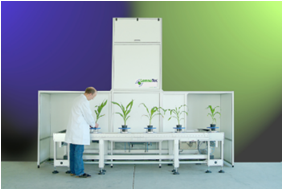
\includegraphics[width=20mm]{conveyor.png}
}
\onslide<2->\subfigure[]{
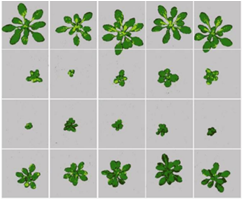
\includegraphics[width=20mm]{sample.png}
}
\onslide<3->\subfigure[]{
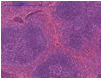
\includegraphics[width=20mm]{mouse.png}
}
\onslide<4->\subfigure[]{
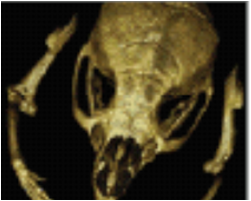
\includegraphics[width=20mm]{organism.png}
}
\end{figure}
\end{frame}

The PODD repository is designed to be used by a number of Australian
research organizations and projects.

Australian Plant Phenomics Facility operates two research centers.

The Plant Accelerator (TPA) at the University of Adelaide is a
high-throughput plant research center. What you see here is a
conveyor belt system. RFID-tagged plants travel in the system and
their images are automatically taken by the imaging stations.

The High Resolution Plant Phenomics Center, the HRPPC, is located
in Canberra. The center focuses on deep phenotyping of plants
using a variety of equipments. Some of them operate on single 
plants in controlled environments, others operate in fields.

The Australian Phenomics Network (APN) is a collaborative research
facility established to provides mouse models for human and animal
diseases. For example, APN uses digital slide scanners to perform
histopathology and organ pathology imaging and analysis.

The Atlas of Living Australia is developing a biodiversity 
information portal for Australia. Collaboration with ALA is 
also one of PODD's goals.

\begin{frame}{Data Management Requirements}
\begin{overprint}
\onslide<1>
\begin{block}{Data capturing}
\begin{tabularx}{\linewidth}{p{35mm}X}
Flow Cytometry & FACS data \\
Histopathology & Zeiss slide images \\
Plant imaging & Lemnatec images, Flourogroscan images, 3D imaging \\
Infrared imaging & FLIR images \\
Chemical measurements & Chlorophyll content, Stomatal conductance \\
Visual observation & Manual reports (plant, mouse phenotypes)\\
$\cdots$ & $\cdots$
\end{tabularx}
\end{block}

\onslide<2>
\begin{block}{Metadata capturing}
\begin{tabularx}{\linewidth}{p{30mm}X}
Project & Project proposal, project plan \\
Investigation & Objectives, design \\
Materials & Lines/genotypes, samples, growth conditions \\
Devices & Specs, settings, versions \\
Processes & Workflows, protocols, variations \\
Measurements & Data, images \\
Analysis & Observations, results \\
$\cdots$ & $\cdots$
\end{tabularx}
\end{block}

\onslide<3>
\begin{block}{Data management tasks}
\begin{itemize}
\item Data distribution \& sharing
\item Data publishing
\item Access control
\item Archival \& versioning
%\item Structure \& metadata
\item Data discovery \& analysis
\item Data integration
\end{itemize}
\end{block}
\end{overprint}
\end{frame}

One of the requirements of PODD is to support data capturing from
various platforms.

As you can see on this slide. there are quite a number of different
ways of imaging and measuring a subject. The challenge here is,
besides capturing the raw image files and observations, capture
sufficient metadata.

Another requirement is managing the metadata. Metadata can be
generated on different levels and at different times. All this
information needs to be recorded in the repository together with
the data.

The above requirements span across the whole range of data management
tasks, including distribution, publishing, access control and versioning. 
In the phenomics domain, the development of a repository that supports 
these tasks need to take diversity and change into consideration.

\begin{frame}{PODD: an ontology-driven repository}
\begin{block}{Goals}
    \begin{itemize}
        \item Acquisition and storage of large volumes of data
        \begin{itemize}
        	%\item Different platforms \& different formats
        	\item Distribution, access control, versioning, etc.
	    \end{itemize}
        \item Data conxtualization
        \begin{itemize}
			\item Logical organization
        	\item Provenance tracking
			\item Discovery \& integration
        \end{itemize}
        \item Prepare for change
        \begin{itemize}
        	\item Changes in domain model
        \end{itemize}
    \end{itemize}
\end{block}
\pause
\begin{block}{Approach}
    \begin{itemize}
        \item An ontology-driven approach
        \item \textbf{Ontologies as the domain model}
        \item Benefits: flexibility \& extensibility
    \end{itemize}
\end{block}
\end{frame}

So, the goals of developing the PODD repository is to support the
above data management tasks for the phenomics community.

After our initial study, we realized that the traditional
database-driven approach may not be the best way of doing it. We
will come and revisit this point later.

Ontologies are a formal representation of a particular application
domain. Besides being a controlled vocabulary that define important
concepts and relations, an ontology can also define complex constraints
on these concepts and relations, making it a very expressive
conceptualization of the domain.

Compared to database schemas, ontologies are more open and
extensible. For these reasons, we choose to develop PODD in an
ontology-based approach. In this talk I will focus on describing how
the domain ontology we develop is used in the repository in the
lifecycles of the management of domain objects.

In the following few slides I will quickly introduce a few projects
related to PODD. I'll also briefly introduce the OWL ontology
language.

\section{Related Work}
\begin{frame}{Related Work}
\begin{block}{FuGe -- Functional Genomics Experiment}
    \begin{itemize}
        \item \emph{Material}, \emph{Protocol}, \emph{Data}, etc.
        \item Can be extended to support phenomics
        \item[$\cross$] Defined in UML \& mapped to database schemas -- difficult to extend for new concepts
    \end{itemize}
\end{block}
\pause
\begin{block}{OBI -- Ontology for Biomedical Investigations}
    \begin{itemize}
        \item \textit{``An integrated ontology for the description of life-science and clinical
        investigations.''}
        \item Comprehensive: 2,600+ classes, 10,000+ axioms
        \item[$\cross$] Complex, computationally ($\mathcal{SHOIN}(D)$)
    \end{itemize}
\end{block}
\end{frame}

FuGe is a UML and database based conceptual model for functional
genomics experiments. It models important domain concepts such as
material, protocol and data and how they relate to each other. 
The model is defined as UML class diagrams and mapped to database 
schemas, as a result, FuGe may be difficult to extend.

The OBI ontology - ontology for biomedical investigation is a
comprehensive but complex ontology. It defines domain concepts 
starting from a very high abstract level. As a result, it is quite 
big, containing about 26 hundred classes and 10 thousand logic
axioms. It is also computationally expensive. We need to performing 
reasoning repeatedly in PODD, we chose not to use OBI as our domain 
ontology. 

\begin{frame}{Related Work}
\begin{block}{Web Ontology Language (OWL)}
\begin{itemize}
    \item Precise, open \& extensible -- exactly what we need!
    \item Provides core language constructs \& vocabularies for expressing complex ontologies -- \emph{data models}
    \item APIs, query engines \& automated reasoners available
\end{itemize}
\end{block}
\begin{block}{Fedora Commons}
\begin{itemize}
	\item Mature open-source digital repository software
	\item Modular \& extensible
	\item Widely used 
\end{itemize}
\end{block}
\end{frame}

The Web Ontology Language is the ontology language with a precise semantics 
and is designed to be open and extensible. For example, OBI is developed
in OWL. It provides language constructs to define domain concepts and relations
and axioms on them. 

The three main ingredients in OWL are classes, predicates and individuals. 
For example, Human can be defined as a class; hasParent can be defined as
a predicate and Aristotle can be defined as an individual. 

Quite a few open-source APIs, query engines and reasoners are available for OWL. 

Fedora Commons is an open-source digital contents management system. It's designed
to be modular and extensible so that it can be used with a variety of plugins
and configurations. It's a very mature software and has been widely used 
to implement institution-wide repository systems.

\section{The PODD Ontology}
\begin{frame}{The PODD Ontology}
\begin{block}{Modeling essentials}
%    \begin{itemize}
%    \item Domain entities
%        \begin{itemize}
%        \item Abstract concepts
%        \item Concrete objects
%        \end{itemize}
%    \item Domain entities defined using OWL \emph{ontologies}
%    \end{itemize}
%\end{block}
%\pause
%\begin{block}{Modeling in OWL}
    \begin{itemize}
    \item Domain concepts -- \emph{OWL classes}
    \item Inter-concept relations -- \emph{OWL predicates} \& \emph{OWL restrictions}
    \item Concrete domain objects -- \emph{OWL Individuals}
    \item Comments, descriptions -- \emph{OWL annotations}
    \end{itemize}
\end{block}
\pause
\begin{block}{Benefits}
	\begin{itemize}
	\item Extensibility through inheritance
	\item Reuse \& integration through \textbf{ontology mapping} \& \textbf{ontology annotation}
		\begin{itemize}
		\item Gene Ontology, Plant Ontology, etc.
		\end{itemize}
	\end{itemize}
\end{block}
\end{frame}

In the same spirit of FuGe and OBI, the PODD ontology defines 
essential domain concepts so that we can describe concrete domain
objects. These concepts and objects are defined using OWL ontologies
and RDF triples.

%\begin{frame}{The Ontology-driven Approach}
%\begin{block}{Benefits}
%    \begin{itemize}
%    \setlength{\itemsep}{6pt}
%    \item<1-> Greater extensibility
%        \begin{itemize}
%        \item New concepts/relations can be easily added/modified
%        \end{itemize}
%    \item<2-> Better reuse \& integration
%        \begin{itemize}
%        \item Ontologies are \emph{open}
%        \item Other ontologies can be integrated
%        \begin{itemize}
%        	\item Class, property \& individual \textbf{mapping}
%			\item Ontological \textbf{annotations}
%        \end{itemize}
%        \end{itemize}
%    \item<3-> Balance between expressivity \& reasoning complexity
%        \begin{itemize}
%        \item Formal semantics enables automated query \& analysis
%        %\item Off-the-shelf tools available
%        \end{itemize}
%    \end{itemize}
%\end{block}
%\end{frame}

The ontology-based approach has a number of benefits. 

Firstly, the repository can be more extensible. In PODD abstract
domain concepts are stored in the repository as well. After we've 
defined the domain ontology, concepts and properties can be extended 
to create new ones. In such a way new concepts and relations
can be added more easily than if the information is stored in a database.

Note here that concept and object definitions are all versioned so
we can freely modify an concept without affecting existing objects.

An ontology-based repository is also better in terms of reuse and integration.
Ontologies are designed to be shared so when you make your ontology available,
you share your model. When you publish your instance data, concrete domain data
is shared. So integration can happen on multiple levels. 

\begin{frame}{The PODD Ontology -- Overview}
\vspace{-12pt}
 \begin{figure}[t]
  \begin{center}
  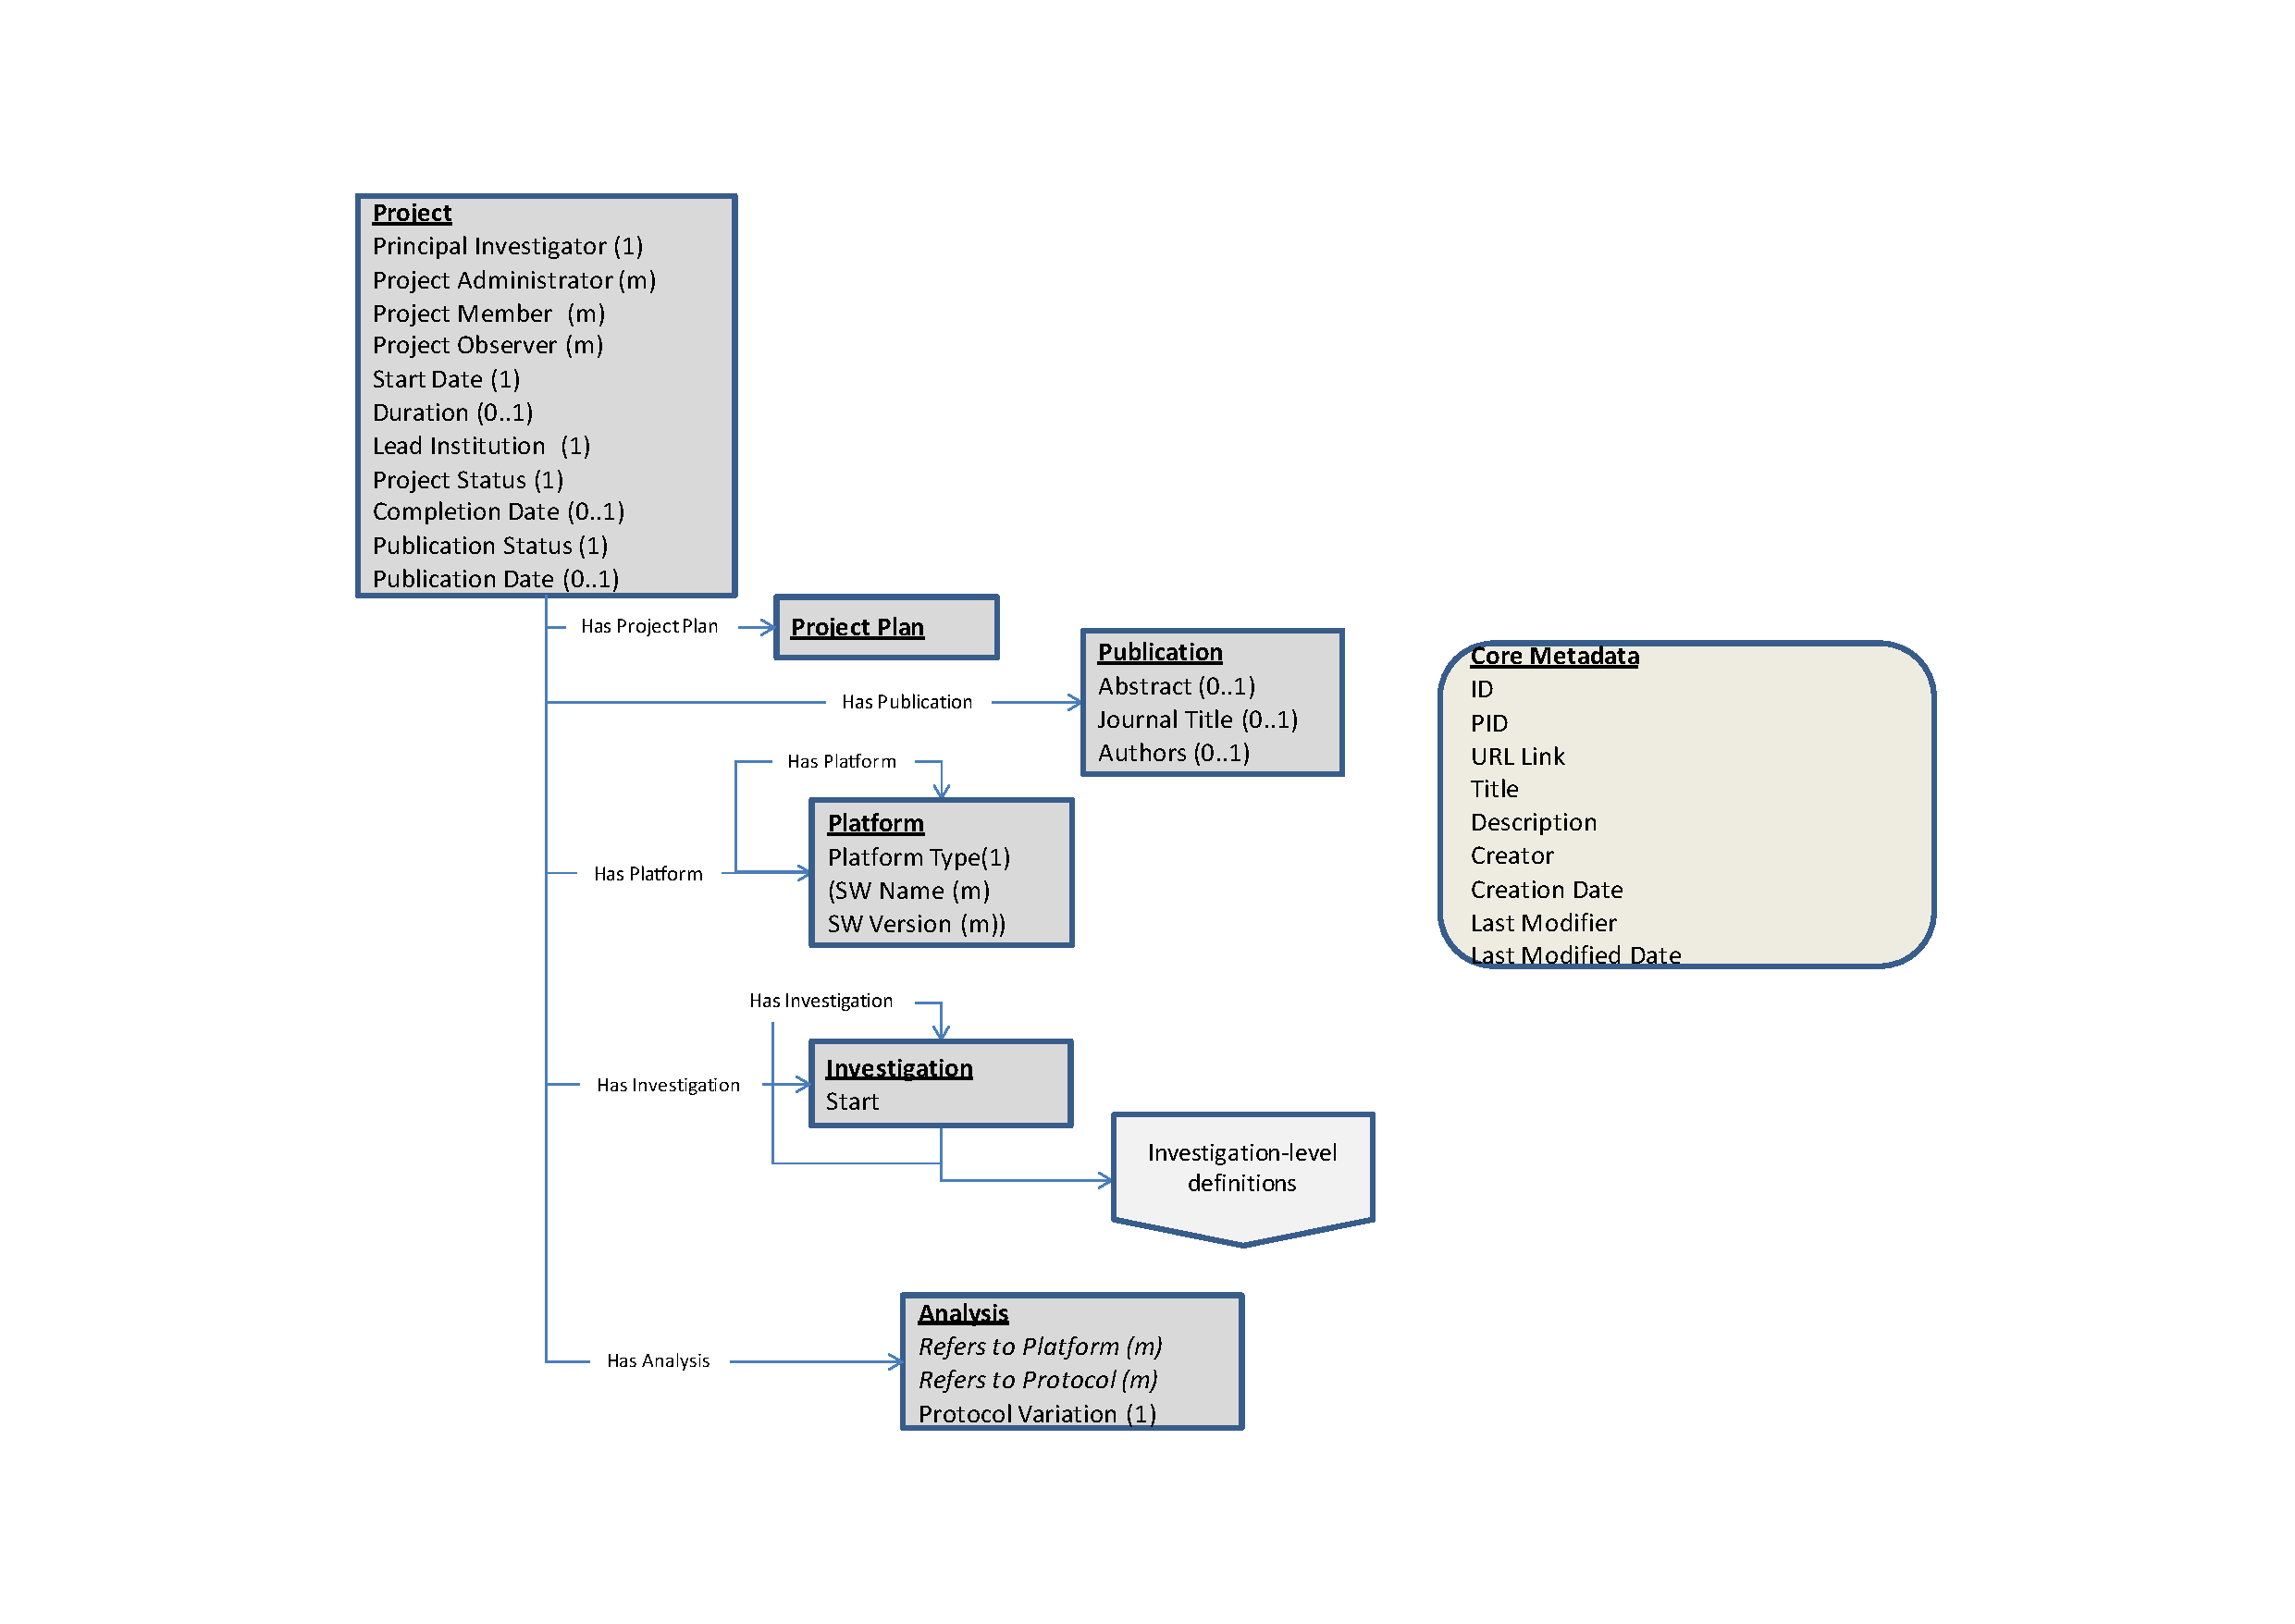
\includegraphics[trim=48mm 30mm 38mm 20mm, clip, width=112mm]{model.pdf}
   \end{center}
  \label{fig:ont}
 \end{figure}
\end{frame}

In this slide we show how some high-level concepts are logically
connected in the PODD domain model. Project is the top-level concept
with a bunch of attributes. It is also connected to some other
concepts like ProjectPlan, Platform and Investigation. Each of these
concepts also should have a number of core metadata attributes.

The concepts here are organized in a tree-like structure. What is not
shown on this slide is cross references between concepts. They are
useful when a particular object is referred to by some other objects.

\begin{frame}{The PODD Ontology -- An Example}
\begin{example}{The \textbf{\emph{Project}} concept}
    \begin{itemize}
    \item The top-level concept
    \item Constraints on inter-object relations \& attributes
    \end{itemize}
    \pause
    {\small
    \begin{align*}
    Project &\sqsubseteq~ =~ 1~ hasProjectPlan \sqcap \forall hasProjectPlan.ProjectPlan\\
            &\sqsubseteq~ \geq~ 1~ hasInvestigation \sqcap \forall hasInvestigation.Investigation\\
            &\sqsubseteq~ =~ 1~ hasStartDate \sqcap \forall hasStartDate.\textit{xsd:date}\\
            &\sqsubseteq~ \leq~ 1~ hasPublicationDate \sqcap \forall hasPublicationDate.date
    \end{align*}}
\end{example}
\begin{block}{}
    \begin{itemize}
    \item \textcolor{blue}{\textbf{Extensibility}} from inheritance of OWL classes \& predicates
    \end{itemize}
\end{block}
\end{frame}

In this slide I show an incomplete modeling of the top-level concept
in our ontology, the Project. In our model of phenomics, everything starts 
from a research project and all other objects, such as Investigation and
Material are child or descendant objects. 

As you see, we define constraints on attributes and inter-concept relations
of the Project concept. This is how we model all of our concepts.

Shown here are 8 constraints. The first line says that any Project instance must
be mapped to exactly 1 other object by the hasProjectPlan object and this 1 object
must be of type ProjectPlan.

%\begin{frame}{The PODD Ontology}
%\onslide<2->
%\begin{columns}[t]
%\column{.5\textwidth}
%\begin{itemize}
%    \item Inspired by FuGe \& OBI
%    \item Aim: define all \emph{essential} domain concepts, attributes \& relations
%    \item $\sim30$ classes, \\$\sim 80$ predicates, \\$\sim 200$ Axioms
%    \item Faster reasoning, querying, etc.
%\end{itemize}
%\vfill
%\onslide<1->
%\column{.5\textwidth}
%\vspace{-10mm}
% \begin{figure}[t]
%  \begin{center}
%  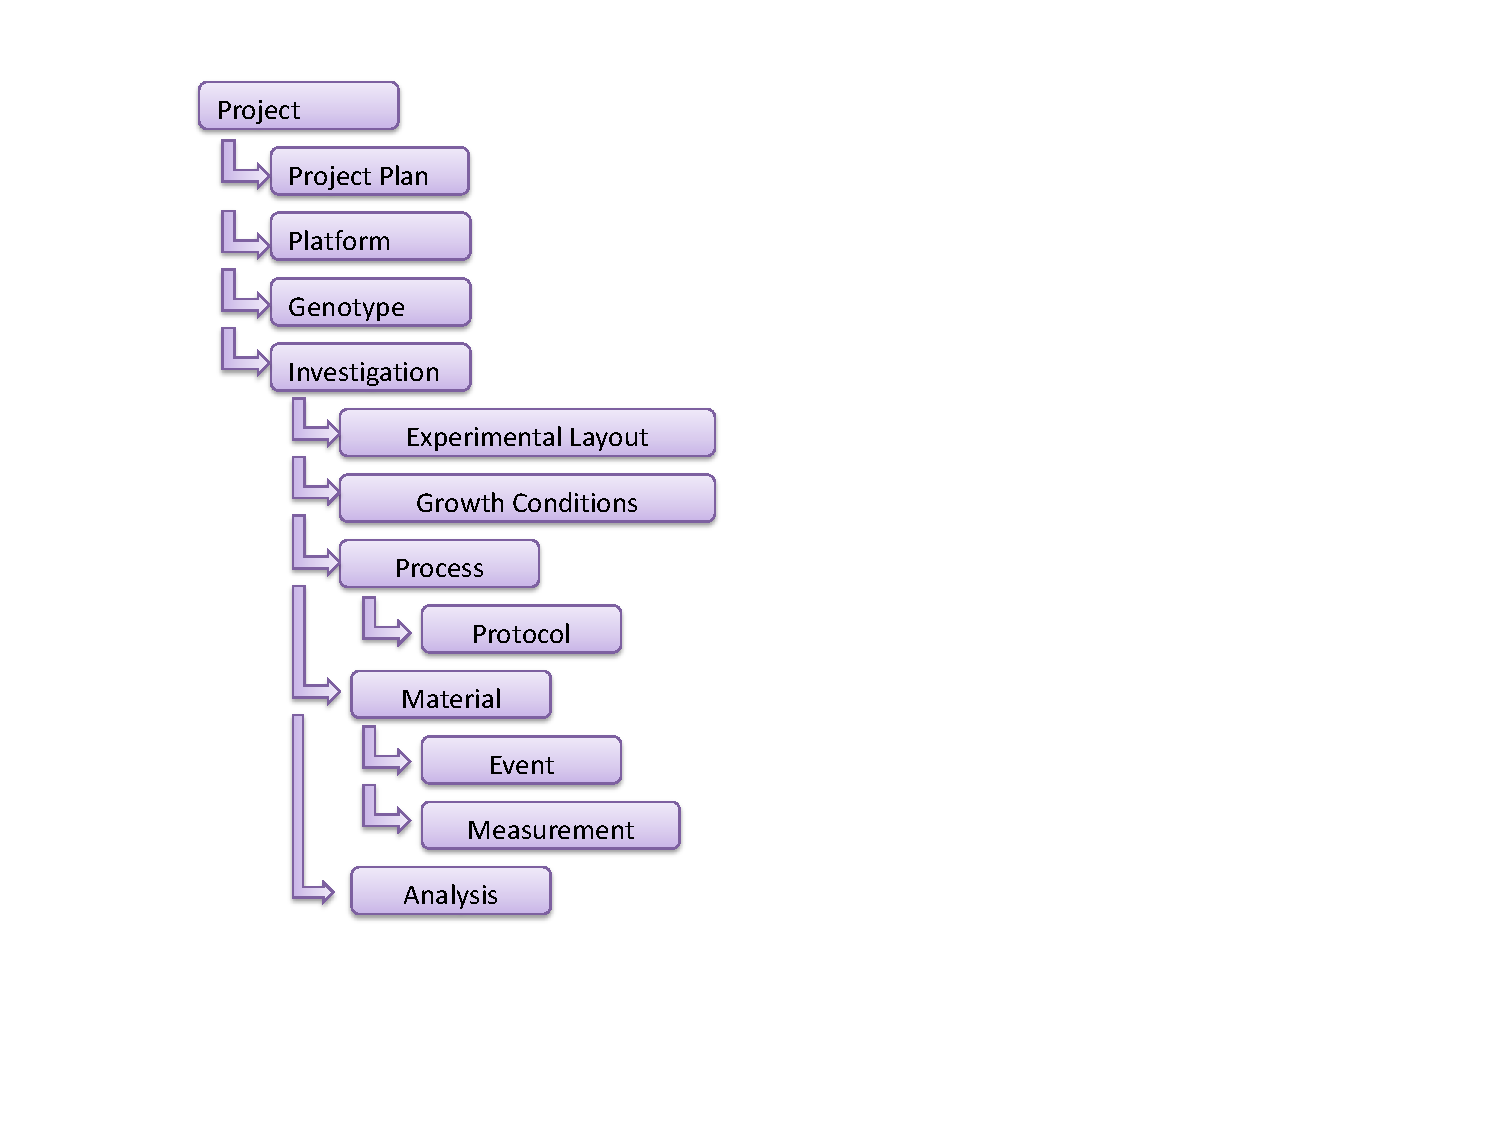
\includegraphics[trim=3mm 26mm 2mm 8mm, clip, height=72mm]{hier.pdf}
%   \end{center}
% \end{figure}
%\end{columns}
%\end{frame}

Here you see a list of important domain concepts in the PODD ontology.
In the development of our ontology we took inspiration from FuGe and OBI
but with the aim that the PODD ontology will cover essential domain
concepts and relations without becoming too complex.

As it currently stands, the ontology defines about 30 OWL classes, 80
predicates and more than 200 logical axioms. 

With this smaller ontology, all core reasoning tasks can be performed
much faster.

\begin{frame}{PODD Ontology -- Roles}
\begin{block}{Ontologies \textbf{\emph{drive}} repository functions}
\begin{list}{}{}
\item[\textcolor{blue}{\textbf{Presentation}}]~\\% Drives the rendering of the web pages
    \begin{itemize}
    \item Object creation, editing, display, etc.
    \end{itemize}
\item[\textcolor{blue}{\textbf{Storage}}] ~\\
	\begin{itemize}
	\item Object (de)serialization to/from ontologies
	\end{itemize}
\item[\textcolor{blue}{\textbf{Validation}}] ~\\%Ontology reasoning performed
    \begin{itemize}
    \item Validation based on concept constraints
    \end{itemize}
\item[\textcolor{blue}{\textbf{Discovery}}] ~\\%Multiple ways of finding information
    \begin{itemize}
    \item Queries using SPARQL
    \item Full-text search
    \end{itemize}
\end{list}
\end{block}
\end{frame}

The PODD ontology is at the center of the repository and it drives quite a lot
of repository functions. All the object metadata is saved as RDF triples
conforming to the ontology definitions. When a web page of creating, editing
or displaying an object is requested, the ontologies are used to determine
what gets displayed and in what way.

The domain objects are serialized into ontologies when they are saved and 
deserialized when they are loaded from the underlying storage.

Before we save and publish an object, the object's triples are validated against
the domain ontology. Objects can be queried and searched for on the RDF triples.

\begin{frame}{The PODD Repository: The High-level Architecture}
\vspace{-10pt}
 \begin{figure}[t]
  \begin{center}
  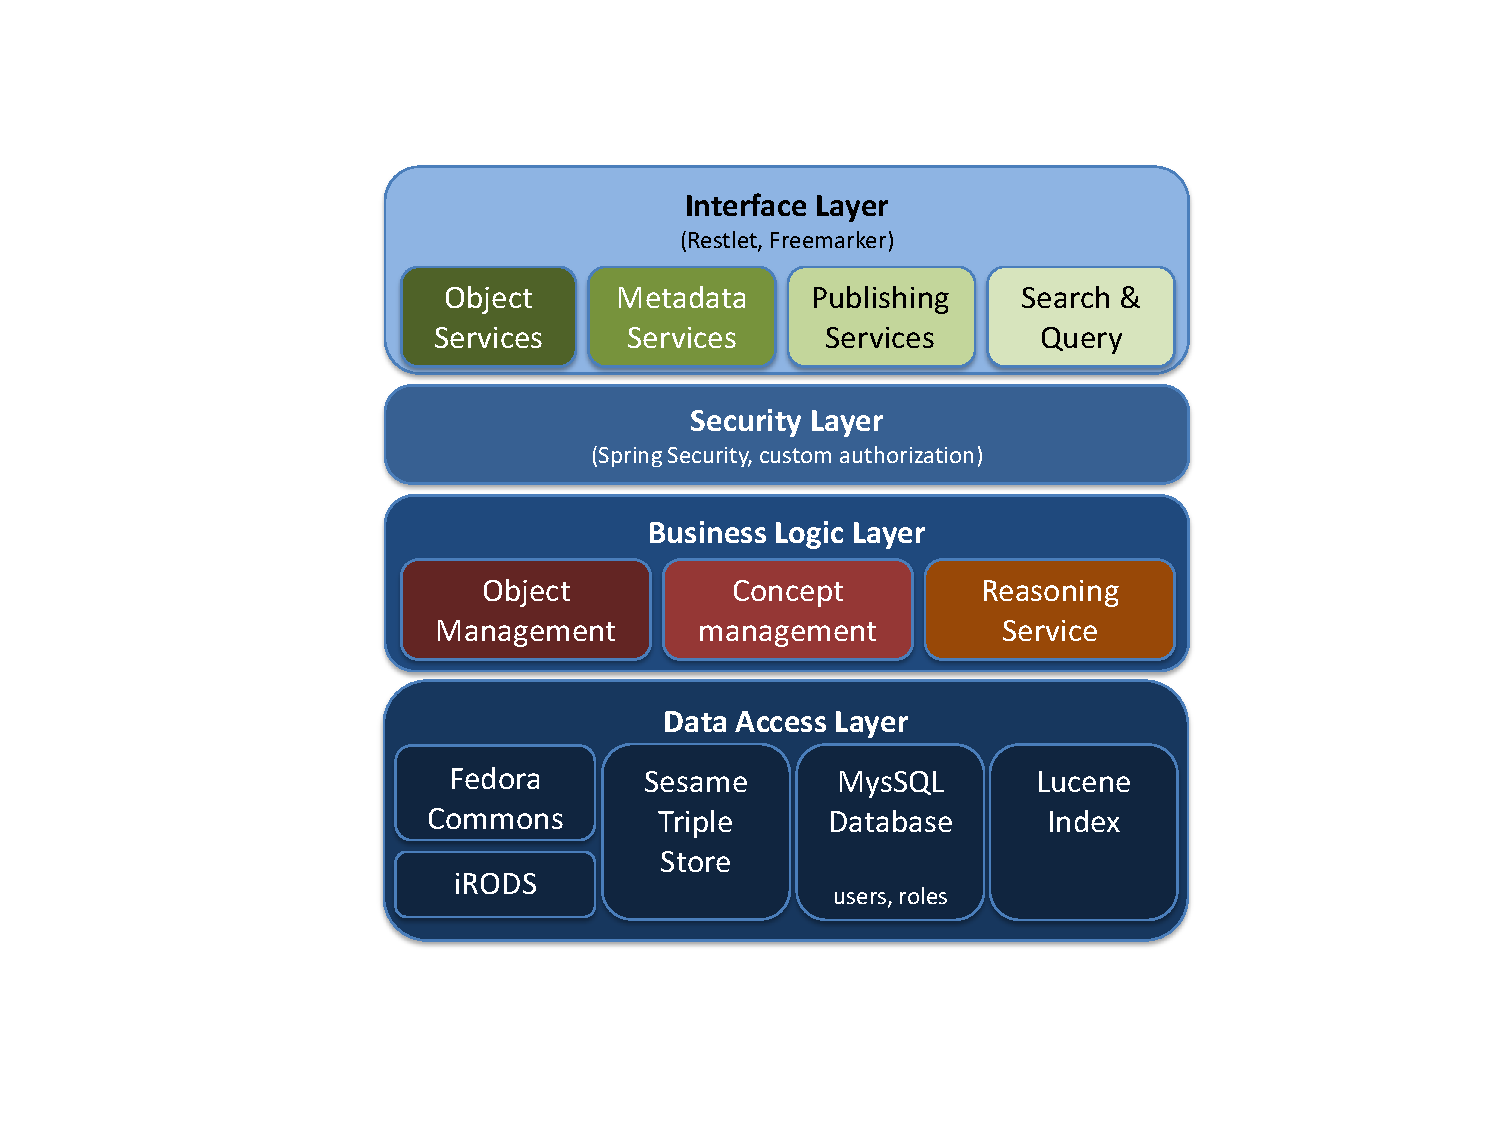
\includegraphics[trim=48mm 30mm 38mm 20mm, clip, width=96mm]{architecture.pdf}
   \end{center}
  \label{fig:arch}
 \end{figure}
\end{frame}

Here you see the high-level architecture of the PODD repository. 
We take a layered approach in designing and developing the system.

The data access layer at the bottom is responsible for 
serializing and deserializing concepts and objects in 
the underlying storage. Objects and their metadata are
stored in Fedora Commons, a very widely-used digital
contents repository software system. iRODS is a federated 
data storage software that can be plugged into Fedora
Commons as a storage module. We use iRODS to store the
Fedora datastreams.

Object definitions in RDF will be stored in a Sesame triple 
store and a Lucene index so that we can query and search for
information. We also use databases to store information
about users, access rights and some other things.

The business logic layer is responsible for managing the 
lifecycles and interactions of objects and concepts. OWL
reasoning is a central component of this layer as we use
ontologies in all sorts of data management tasks.

On top of that is the security layer, which handles authentication
and authorization. We have a fine-grained authorization module
where access rights are granted on a per-user and per-project basis.

At the top of the stack is the interface layer. PODD is a web-based
system so all functionality can be accessed through a browser as
well as through API calls. 

\section{Conclusion}
\subsection*{ }
\begin{frame}{Conclusion}
\begin{block}{To recap}
\begin{itemize}
\item Large amounts of data need to be managed
    \begin{itemize}
    \item There is a need for data archival, storage \& discovery
    \end{itemize}
\item Current approaches lacking/inadequate/inflexible
    \begin{itemize}
    \item Emerging processes, platforms, technologies require a extensible conceptual framework
    \end{itemize}
\item An ontology-driven architecture as the foundation of PODD
    \begin{itemize}
    \item Ontologies as the domain model
    \item Extensible \& open
    \end{itemize}
\end{itemize}
\end{block}
\end{frame}

As a result, in PODD we propose an ontology-driven architecture
for developing extensible data repositories. In this framework
databases take a back seat and ontologies are used to describe
the domain. We believe it is more extensible, flexible and open.

\begin{frame}{Conclusion}
\begin{block}{Where we are now}
\begin{itemize}
\item PODD ontology for phenomics research
\item Development of basic repository functionality
\item Development of PODD web interface
\end{itemize}
\end{block}
\pause
\begin{block}{What's next}
\begin{itemize}
\item Development of batch data import/export processes
\item Development of object discovery services
\item Integration with Shibboleth authentication 
\item \textcolor{gray}{Exposing data for discovery}
\item \textcolor{gray}{Integrating with other data sources}
\end{itemize}
\end{block}
\end{frame}

So far we have developed an ontology for plant and
mouse phenomics research. Centered around this ontology
we have implemented basic repository functionalities
including object storage, versioning, validation, 
publishing, searching and presentation generation. 

In future we will implement a number of tasks that are
important for phenomics research. These include data
import and export, object discovery and more flexible
authentication with Shibboleth.

We will also be looking at how we can expose data in
the PODD repository to external world and how they 
can be integrated with existing datasets.

\begin{frame}
	\frametitle{}
    \begin{center}
\Huge \textsc{\textcolor{blue}{\textbf{Thank You!}}}
\end{center}
\vspace{+20pt}
\begin{block}{Acknowledgment}
Faith Davies, Gavin Kennedy, Jane Hunter @
eResearch Lab, School of ITEE, UQ
\end{block}
\end{frame}

\end{document}
